%% 
%% Copyright 2007-2020 Elsevier Ltd
%% 
%% This file is part of the 'Elsarticle Bundle'.
%% ---------------------------------------------
%% 
%% It may be distributed under the conditions of the LaTeX Project Public
%% License, either version 1.2 of this license or (at your option) any
%% later version.  The latest version of this license is in
%%    http://www.latex-project.org/lppl.txt
%% and version 1.2 or later is part of all distributions of LaTeX
%% version 1999/12/01 or later.
%% 
%% The list of all files belonging to the 'Elsarticle Bundle' is
%% given in the file `manifest.txt'.
%% 
%% Template article for Elsevier's document class `elsarticle'
%% with harvard style bibliographic references

\documentclass[preprint,12pt,authoryear]{elsarticle}

%% Use the option review to obtain double line spacing
%%\documentclass[authoryear,preprint,review,12pt]{elsarticle}

%% Use the options 1p,twocolumn; 3p; 3p,twocolumn; 5p; or 5p,twocolumn
%% for a journal layout:
%% \documentclass[final,1p,times,authoryear]{elsarticle}
%%\documentclass[final,1p,times,twocolumn,authoryear]{elsarticle}
%% \documentclass[final,3p,times,authoryear]{elsarticle}
%% \documentclass[final,3p,times,twocolumn,authoryear]{elsarticle}
%% \documentclass[final,5p,times,authoryear]{elsarticle}
%%\documentclass[final,5p,times,twocolumn,authoryear]{elsarticle}

%% For including figures, graphicx.sty has been loaded in
%% elsarticle.cls. If you prefer to use the old commands
%% please give \usepackage{epsfig}

%% The amssymb package provides various useful mathematical symbols
\usepackage{amssymb}
%% The amsthm package provides extended theorem environments
%% \usepackage{amsthm}

%% The lineno packages adds line numbers. Start line numbering with
%% \begin{linenumbers}, end it with \end{linenumbers}. Or switch it on
%% for the whole article with \linenumbers.
%% \usepackage{lineno}
\usepackage{pgfplotstable,filecontents}
\usepackage{hyperref}
\hypersetup{
    colorlinks=false,
    pdfborder={0 0 0},
}
\usepackage{amsmath}
\usepackage{placeins}  % for \FloatBarrier
\usepackage{svg}
\journal{Ocean Engineering}

\begin{document}

\begin{frontmatter}

    %% Title, authors and addresses

    %% use the tnoteref command within \title for footnotes;
    %% use the tnotetext command for theassociated footnote;
    %% use the fnref command within \author or \affiliation for footnotes;
    %% use the fntext command for theassociated footnote;
    %% use the corref command within \author for corresponding author footnotes;
    %% use the cortext command for theassociated footnote;
    %% use the ead command for the email address,
    %% and the form \ead[url] for the home page:
    %% \title{Title\tnoteref{label1}}
    %% \tnotetext[label1]{}
    %% \author{Name\corref{cor1}\fnref{label2}}
    %% \ead{email address}
    %% \ead[url]{home page}
    %% \fntext[label2]{}
    %% \cortext[cor1]{}
    %% \affiliation{organization={},
    %%            addressline={}, 
    %%            city={},
    %%            postcode={}, 
    %%            state={},
    %%            country={}}
    %% \fntext[label3]{}

    \title{System identification of a physics informed manoeuvring model for better predictions in wind conditions}

    %% use optional labels to link authors explicitly to addresses:
    %% \author[label1,label2]{}
    %% \affiliation[label1]{organization={},
    %%             addressline={},
    %%             city={},
    %%             postcode={},
    %%             state={},
    %%             country={}}
    %%
    %% \affiliation[label2]{organization={},
    %%             addressline={},
    %%             city={},
    %%             postcode={},
    %%             state={},
    %%             country={}}

    \author[1,2]{Martin Alexandersson\corref{cor1}%
        %\fnref{fn1,fn3}
    }
    \ead{maralex@chalmers.se}
    \author[1]{Wengang Mao}
    \author[1]{Jonas W. Ringsberg}
    \author[2]{Martin Kjellberg}


    \affiliation[1]{organization={Dept. of Mechanics and Maritime Sciences, Division of Marine Technology, Chalmers University of Technology},%Department and Organization
        addressline={Hörsalsvägen 7A},
        city={Gothenburg},
        postcode={41296},
        country={Sweden}}


    \affiliation[2]{organization={Research Institutes of Sweden (RISE)},%Department and Organization
        addressline={Chalmers tvärgata 10},
        city={Gothenburg},
        postcode={41296},
        country={Sweden}}

    \cortext[cor1]{Corresponding author}

    \begin{abstract}
        % Move 1 - Background/introduction/situation

System identification offers ways to identify proper models to describe a ship's dynamics in real operational conditions, but also poses some major challenges, such as multicollinearity and generality of the identified model. 
% Move 2 - Present research/purpose
This paper proposes a new physics informed manoeuvring model, where a deterministic semi-empirical rudder model has been added, to guide the identification towards a physically correct model.  
This is an essential building block to solve ship manoeuvring modelling uncertainties from wind, waves, and currents, which are either added for a real sea conditions or important to model for ships with wind-assisted propulsion.
In the physics informed manoeuvring modeling framework, a systematical procedure is developed to establish various force/motion components within the manoeuvring system by the inverse dynamics regression. 
% Move 3 - Methods/materials/subjects/procedures
To assess the physical correctness, a reference model, is first established via parameter identification on virtual captive zigzag tests. The reference model is assumed to resemble the physically correct kinetics.  on  model tests for: the physics informed model, as well as an uninformed mathematical Abkowitz model -- for compariso

% Move 4 - Results/findings

All of the models predicted the zigzag tests with satisfactory agreement and can thus indeed be considered as being mathematically correct; However, the introduction of a semi-empirical rudder model seems to have guided the identification towards a more physically correct calm water hydrodynamic model, with lower multicollinearity and better generalization. The physics informed model predicted forces and moments that were much more in agreement to the reference model than the Abkowitz model did, and can thus be considered as the more physically correct model. 

% Move 5 - Discussion/conclusion/significance


    \end{abstract}

    %%Graphical abstract
    %\begin{graphicalabstract}
    %    %\includegraphics{grabs}
    %\end{graphicalabstract}
    %
    %%%Research highlights
    %\begin{highlights}
    %    \item Research highlight 1
    %    \item Research highlight 2
    %\end{highlights}

    \begin{keyword}
    Physics-informed manoeuvring model; Inverse dynamics; Wind-assisted propulsion; System identification;  Multicollinearity.
        %% keywords here, in the form: keyword \sep keyword

        %% PACS codes here, in the form: \PACS code \sep code

        %% MSC codes here, in the form: \MSC code \sep code
        %% or \MSC[2008] code \sep code (2000 is the default)

    \end{keyword}

\end{frontmatter}

%% \linenumbers

%% main text
\section{Introduction}
\label{sec:introduction}
Prediction of ship maneuverability, which relies on accurate mathematical models to simulate, e.g., Turning Circle Maneuver, Zig-zag Maneuver, etc., is essential for both ship design and intelligent ship navigation. The mathematical ship maneuverability models require inputs of hydrodynamic forces and moments acting on the ship hull, commonly known as “hydrodynamic coefficients”, “maneuvering coefficients” or “maneuvering derivatives” in non-dimensional form. Various approaches have been proposed to derive those non-dimensional hydrodynamic coefficients by different parameter identification methods, such as simple regression, SVM, Kalman filter, and inverse dynamics, such as Tongtong et al. (2020), Zou et al. (2022), Alexandersson et al. (2021, 2022, 2023), ... In Tongtong et al. (2021) and Alexandersson et al. (2022), different mathematical models have been investigated to describe the most accurate and robust ship maneuvering simulations, also referred to the system identification methods.

However, it should be noted that most research activities aimed to identify a ship's maneuverability mathematical models are built on a ship's simulation data, i.e., a type of inverse engineering to find the model used to simulate the ship maneuvering data. While for practical application, the only reliable source of hydrodynamic coefficients is a model test (ABS 2006), which should also be validated later by full scale test /sea trial). Therefore, several knowledge gaps should be investigated to researched to close the gap between purely simulation-based PIM and generic application of the identified MM model from model to actual usage:
\begin{enumerate}
    \item the parameter identification method based on the simulation data can effectively estimate the hydrodynamic coefficients since the exact "psychical" mathematical model is assumed known. In real cases/applications, the mathematical model is just the simplification of real physics (from VCT, model test, sea trials, or full-scale tests), while the complexity of hydrodynamics involved in vessel maneuvering will greatly challenging the simplified empirical mathematical methods without carefully considering the actual physics inside hydrodynamic coefficients and their interactions (ABS 2006).
    \item if some "actual" data (not simulation data) is used to identify the mathematical model, the PIT may be able to give a good prediction of tested maneuvering trajectories, but the identified mathematical maneuverability model may lack of generalization. It means that the model can only be used to predict the ship's maneuverability under the test scenarios, because the mathematical models cannot capture physics in generic maneuvering scenarios.
    \item to make the method worse, when using non-simulated data for system identification of maneuverability models, the identified model may give wrong physics, i.e., non-physical hydrodynamic forces regressed from the model. Obviously, for this case, the mathematical model identified based on tests from Turning Circle Maneuver can be only reliably used to predict a ship's maneuverability under turning circle tests but not for the zig-zag tests, and vice verse. In some special case, the prediction can be limited to replicating similar test conditions, such as zig-zag tests at certain angles.
    \item the prediction of ship maneuverability from the mathematical model (established from ideal conditions such as model tests) is required to be validated/verified by "real" environment conditions, such as sea trials or full-scale tests. The drift caused by wind/current that are not considered in the mathematical maneuverability model will cause completely failure of the identified model applied for real prediction cases.
\end{enumerate}

Therefore, this study aims to propose a holistic approach to integrate some physical hydrodynamic terms in the mathematical maneuverability model for a more generic ship maneuverability system identification. This approach can make use of test data in ideal conditions to establish a physics-guided mathematical maneuverability model, which can predict a ship's maneuverability under more generic maneuvering scenarios.
%% Literature review here...

% Background...
% * Other people are identifying standard manoeuvres
% * 
The present paper highlights the difficulties in identifying a pure mathematical manoeuvring model -- such as the Abkowitz model -- from calm water manoeuvring test motions for a model that should generalize to have physically correct hydrodynamics also in wind conditions. 

% Objective...
% Use VCT CFD to validate the physics
In order to mitigate these difficulties, more prior knowledge about the rudder hydrodynamics has been added to the model. A new semi-empirical rudder model is therefor introduced in this paper, based on semi-empirical formulas from the literature. The identified models with the pure mathematical structure and the introduced semi-empirical rudder are assessed with: manoeuvring model tests in calm water, CFD calculated virtual captive tests (VCT), and an idealized wind condition.

In this paper the manoeuvring models are first introduced in \autoref{sec:theory} -- this is a reference section that may be skipped during the first read of this paper -- followed by methodology in \autoref{sec:methodology} -- about the parameter identification techniques; the case study ship and datasets are then described in \autoref{sec:case_study}, followed by results (\autoref{sec:results}), discussion (\autoref{sec:discussion}), and conclusions (\autoref{sec:conclusions}).

%
%
%
\section{Proposed physics-informed ship manoeuvring model}
\label{sec:ship_models}
Two different modular manoeuvring models are used in this paper, the physics informed model (PI model), and the physics uninformed model (PU model); They both have identical prediction models for the hull and propeller forces, but different models for the rudder forces. The PI model has a new deterministic semi-empirical rudder model -- proposed in this paper (see \autoref{sec:semiempirical_rudder_model}). The PU model instead has a data driven mathematical rudder model. 
Except the changed rudder models, the manoeuvring models are similar to the MMG model \citep{yasukawa_introduction_2015}, with some minor enhancements that are presented in the next section.
\FloatBarrier
\subsection{Basic Manoeuvring Model}
\label{sec:models}
\subsection{Models}
\label{sec:models}
The kinematics of the manoeuvring models are described by \autoref{eq:X}-\autoref{eq:N}, where $X_D$, $Y_D$, and $N_D$ describe the total external forces and moments acting on the ship in the surge, sway, and yaw degrees of freedoms.
\begin{equation}
    \label{eq:X}
    m \left(\dot{u} - r^{2} x_{G} - r v\right) = X_{D} + X_{\dot{u}} \dot{u}
\end{equation}
%
\begin{equation}
    \label{eq:Y}
    m \left(\dot{r} x_{G} + \dot{v} + r u\right) = Y_{D} + Y_{\dot{r}} \dot{r} + Y_{\dot{v}} \dot{v}
\end{equation}
%
\begin{equation}
    \label{eq:N}
    I_{z} \dot{r} + m x_{G} \left(\dot{v} + r u\right) = N_{D} + N_{\dot{r}} \dot{r} + N_{\dot{v}} \dot{v}
\end{equation}

The external forces are expressed in a modular way similar to the MMG model \citep{yasukawa_introduction_2015},
% Components:
\begin{equation}
    \label{eq:X_D}
    X_{D} = X_{H} + X_{P} + X_{R}
\end{equation}
%
\begin{equation}
    \label{eq:Y_D}
    Y_{D} = Y_{H} + Y_{P} + Y_{R} + Y_{RHI}
\end{equation}
%
\begin{equation}
    \label{eq:N_D}
    N_{D} = N_{H} + N_{P} + N_{R} + N_{RHI}
\end{equation}
where the subscripts: H, P, R, and RHI represent contributions from: hull, propellers, rudders, and rudder hull interaction.

% Hull:
The hull forces are expressed with the following polynomials expressed in prime system units,
\begin{equation}
    \label{eq:X_H}
    {X_H'} = {X_{0}'} + {X_{rr}'} {r'}^{2} + {X_{u}'} {u'} + {X_{vr}'} {r'} {v'} + {X_{vv}'} {v'}^{2}
\end{equation}
%
\begin{equation}
    \label{eq:Y_H}
    {Y_H'} = {Y_{0}'} + {Y_{r}'} {r'} + {Y_{v}'} {v'} + {\cancel{Y_{rrr}}'} {r'}^{3} + {\cancel{Y_{vrr}}'} {r'}^{2} {v'} + {\cancel{Y_{vvr}}'} {r'} {v'}^{2} + {\cancel{Y_{vvv}}'} {v'}^{3}
\end{equation}
%
\begin{equation}
    \label{eq:N_H}
    {N_H'} = {N_{0}'} + {N_{r}'} {r'} + {N_{v}'} {v'} + {\cancel{N_{rrr}}'} {r'}^{3} + {\cancel{N_{vrr}}'} {r'}^{2} {v'} + {\cancel{N_{vvr}}'} {r'} {v'}^{2} + {\cancel{N_{vvv}}'} {v'}^{3}
\end{equation}
%Propellers:
The propeller forces are expressed as,
\begin{equation}
    \label{eq:X_P}
    X_{P} = X_{P port} + X_{P stbd}
\end{equation}
%
\begin{equation}
    \label{eq:Y_P}
    Y_{P} = 0
\end{equation}
%
\begin{equation}
    \label{eq:N_P}
    N_{P} = N_{P port} + N_{P stbd}
\end{equation}
The surge forces from the propellers are calculated as the propeller thrust times a thrust deduction coefficient $X_{thrust}=(1-t)$ as shown in for the port propeller in \autoref{eq:X_P_port} and a small yawing moment contribution as seen in \autoref{eq:N_P_port}.
\begin{equation}
    \label{eq:X_P_port}
    X_{P port} = X_{Tport} T_{port}
\end{equation}
\begin{equation}
    \label{eq:N_P_port}
    N_{P port} = - X_{P port} y_{p port}
\end{equation}

%Rudder hull interaction:
There is an interaction effect between the rudder and hull. The flow in the ship's aft is influenced by the rudder -- which generates lift on the hull surface -- so that forces from rudder actions are generated both on the rudder and on the hull. This effect is modelled by the coefficients $\alpha_H$ and $x_H$ as seen in \autoref{eq:Y_RHI} and \autoref{eq:N_RHI}.
\begin{equation}
    \label{eq:Y_RHI}
    Y_{RHI} = Y_{R} a_{H}
\end{equation}
%
\begin{equation}
    \label{eq:N_RHI}
    N_{RHI} = N_{R} x_{H}
\end{equation}

In this paper two different rudder models are used for the rudder forces: a pure mathematical rudder model and a semi-empirical rudder model.
%
\subsection{Proposed physical/semi-empirical rudder model}
\label{sec:semiempirical_rudder_model}
The semi-empirical rudder model is a lifting line model. The surge and sway force are expressed as: rudder lift $L_R$, and rudder drag $D_R$, which are projected on the ship through the rudder inflow angle $\alpha_f$ (see \autoref{eq:X_R_semiempirical} and \autoref{eq:Y_R_semiempirical}).
This angle is a sum of the initial inflow to the rudder at a straight course $\gamma_0$ and the inflow to the rudder $\gamma$ due to: propeller induced speed, drift angle, and yaw rate of the ship; as seen in \autoref{eq:gamma_semiempirical}.
\begin{equation}
    \label{eq:X_R_semiempirical}
    X_{R } = - D_{R } \cos{\left(\alpha_{f } \right)} + L_{R } \sin{\left(\alpha_{f } \right)}
\end{equation}
%
\begin{equation}
    \label{eq:Y_R_semiempirical}
    Y_{R} = D_{R} \sin{\left(\alpha_{f} \right)} + L_{R} \cos{\left(\alpha_{f} \right)}
\end{equation}
%
\begin{equation}
    \label{eq:alpha_f_semiempirical}
    \alpha_{f } = \gamma_{0 } + \gamma_{}
\end{equation}
%
\begin{equation}
    \label{eq:gamma_semiempirical}
    \gamma_} = \operatorname{atan}{\left(\frac{V_{R y}}{V_{R x C}} \right)}
\end{equation}
The transverse velocity at the rudder $V_{Ry}$ is calculated with the ship's yaw rate $r$ and the transverse velocity $v$ multiplied by their flow straightening $\kappa_{rtot}$ and $\kappa_{vtot}$ (\autoref{eq:V_R_y_semiempirical}). The flow straightening has a nonlinear dependency of the geometric inflow angle $\gamma_g$ (\autoref{eq:gamma_g_semiempirical}) as seen in \autoref{eq:kappa_r_tot_semiempirical} and \autoref{eq:kappa_v_tot_semiempirical}, so that the flow straightening may vary for different inflow angles, which is an enhancement compared to the MMG model.
The axial velocity at the rudder $V_{RxC}$, including the velocity of the propeller race is presented in \autoref{sec:velocity_in_the_propeller_slip_stream}.
\begin{equation}
    \label{eq:V_R_y_semiempirical}
    V_{R y} = - \kappa_{r tot} r x_{R} - \kappa_{v tot} v
\end{equation}
%
\begin{equation}
    \label{eq:kappa_r_tot_semiempirical}
    \kappa_{r tot} = \kappa_{r} + \kappa_{r \gamma g} \left|{\gamma_{g}}\right|
\end{equation}
%
\begin{equation}
    \label{eq:kappa_v_tot_semiempirical}
    \kappa_{v tot} = \kappa_{v} + \kappa_{v \gamma g} \left|{\gamma_{g}}\right|
\end{equation}
%
\begin{equation}
    \label{eq:gamma_g_semiempirical}
    \gamma_{g} = \operatorname{atan}{\left(\frac{- r x_{R} - v}{V_{R x C}} \right)}
\end{equation}

The yaw moment is modelled as the sway force times a lever arm $x_R$ as seen in \autoref{eq:N_R_semiempirical}.
\begin{equation}
    \label{eq:N_R_semiempirical}
    N_{R} = Y_{R} x_{R}
\end{equation}
%
%
\subsubsection{Rudder lift}
\label{sec:rudder lift}
With the inspiration from the work of \citet{villa_numerical_2020}, the total rudder lift is calculated as the sum of the lift from the part of the rudder that is covered by the propeller race $L_{RC}$ and the uncovered part $L_{RU}$ as seen in \autoref{eq:L_R_semiempirical}.
\begin{equation}
    \label{eq:L_R_semiempirical}
    L_{R } = L_{R C } + L_{R U }
\end{equation}
The lift forces are calculated with the lift coefficient $C_L$ as seen in \autoref{eq:L_R_U_semiempirical} and \autoref{eq:L_R_C_semiempirical}. These equations are essentially the same except that the lift by the covered part $L_{RC}$ is diminished by the factor $\lambda_R$ (\autoref{eq:lambda_R_semiempirical}) due to the limited radius of the propeller slipstream in the lateral direction \citep{brix_manoeuvring_1993}. A tuning coefficient $C_{Ltune}$ has also been added to these equations.
\begin{equation}
    \label{eq:L_R_U_semiempirical}
    L_{R U } = \frac{A_{R U} C_{L } C_{L tune} V_{R U }^{2} \rho}{2}
\end{equation}
%
\begin{equation}
    \label{eq:L_R_C_semiempirical}
    L_{R C } = \frac{A_{R C} C_{L } C_{L tune} V_{R C }^{2} \lambda_{R } \rho}{2}
\end{equation}
The velocities of the uncovered $V_{RU}$ and covered $V_{RC}$ parts of the rudder are calculated according to \ref{sec:velocity_outside_the_propeller_slip_stream}, and \ref{sec:velocity_in_the_propeller_slip_stream}.

For a none stalling rudder, the lift coefficient $C_L$ is calculated with \autoref{eq:C_L_semiempirical},
\begin{equation}
    \label{eq:C_L_semiempirical}
    C_{L} = \lambda_{gap} \left(\alpha_} dC_{L dalpha} + \frac{C_{DC} \alpha_} \left|{\alpha_}}\right|}{AR_{e}}\right)
\end{equation}
%
\begin{equation}
    \label{eq:alpha_semiempirical}
    \alpha_{} = \\delta + \gamma_{0 } + \gamma_{}
\end{equation}
The effective aspect ratio $AR_e$ accounts for the mirror image effect when the rudder is flush with the hull, where the effective aspect ratio is typically assumed to be twice the geometric aspect ratio $AR_g$ (\autoref{eq:AR_e_semiempirical}) \citep{hughes_tempest_2011}.
The WPCC rudder is however not flush to the hull, so that a gap is created between the rudder and rudder horn for larger rudder angles. This gap reduces the pressure difference between the high and low pressure sides in the upper part of the rudder. \citet{matusiak_dynamics_2021} proposed that the gap effect can be modelled as a reduced aspect ratio. Instead a simpler approach is proposed in the this paper -- based on experience. A factor $\lambda_{gap}$ is introduced, which is calculated according to \autoref{eq:lambda_gap_semiempirical}. The gap effect is only activated above a threshold rudder angle $\delta_{lim}$, and the strength of the gap effect is modelled by a factor $s$ as seen in \autoref{fig:gap}.
\begin{equation}
    \label{eq:lambda_gap_semiempirical}
    C_{gap} = \begin{cases} 1 & \text{for}\: \delta_{lim} > \left|{\delta}\right| \\s \left(- \delta_{lim} + \left|{\delta}\right|\right)^{2} + 1 & \text{otherwise} \end{cases}
\end{equation}
\begin{figure}[h]
    \centering
    \includesvg[width=0.5\columnwidth]{figures/gap_effect.gap.svg}
    \caption{The rudder lift is reduced by the gap between rudder and rudder horn for larger rudder angles.}
    \label{fig:gap}
\end{figure}
The lift slope of the rudder $\frac{\partial C_L}{\partial \alpha}$ is calculated with \autoref{eq:dC_L_dalpha_semiempirical} where $a_0$ is the section lift curve slope (\autoref{eq:a_0_semiempirical}) and $\Omega$ is the sweep angle of the quarter chord line \citep{lewis_principles_1989}.
\begin{equation}
    \label{eq:dC_L_dalpha_semiempirical}
    dC_{L dalpha} = \frac{AR_{e} a_{0}}{\sqrt{\frac{AR_{e}^{2}}{\cos^{4}{\left(\Omega \right)}} + 4} \cos{\left(\Omega \right)} + 1.8}
\end{equation}
%
\begin{equation}
    \label{eq:AR_e_semiempirical}
    AR_{e} = 2 AR_{g}
\end{equation}
%
\begin{equation}
    \label{eq:AR_g_semiempirical}
    AR_{g} = \frac{b_{R}^{2}}{A_{R}}
\end{equation}
%
\begin{equation}
    \label{eq:a_0_semiempirical}
    a_{0 } = 1.8 \pi
\end{equation}
There is also a small nonlinear part to $C_L$ modelled by the cross flow drag coefficient $C_{DC}$ which is calculated for a rudder with squared tip using \autoref{eq:C_D_crossflow_semiempirical} where the taper ratio $\lambda$ is defined as the ratio between the chords at the tip and the root of the rudder (\autoref{eq:lambda__semiempirical}) \citep{hughes_tempest_2011}. 
\begin{equation}
    \label{eq:C_D_crossflow_semiempirical}
    C_{DC} = 1.6 \lambda^{} + 0.1
\end{equation}
%
\begin{equation}
    \label{eq:lambda__semiempirical}
    \lambda} = \frac{c_{t}}{c_{r}}
\end{equation}
%
%
\subsubsection{Rudder drag}
\label{sec:rudder_drag}
The total rudder drag $D_R$ is calculated as a sum of the contributions from the parts covered and uncovered by the propeller as seen in \autoref{eq:D_R_semiempirical}.
\begin{equation}
    \label{eq:D_R_semiempirical}
    D_{R } = 0.5 \rho \left(A_{R C} C_{D C } V_{R C }^{2} + A_{R U} C_{D U } V_{R U }^{2}\right)
\end{equation}
The drag coefficients: $C_{DC}$, and $C_{DU}$ are calculated with semi-empirical formulas according to \autoref{sec:CD}.


%
\subsection{Prime system}
\label{sec:prime_system}
\subsection{Prime system}
\label{sec:prime_system}
Some equations in this paper are expressed using non dimensional units with the prime system, denoted by the prime symbol ($'$). The quantities are expressed in the prime system, using the denominators in \autoref{tab:prime_system}.
\begin{table}[h!]
    \centering
    \caption{Scalings with prime system}
    \label{tab:prime_system}
    \pgfplotstabletypeset[col sep=comma,
        columns={Physical quantity,SI unit,Prime system},
        columns/SI unit/.style={string type},
        columns/Physical quantity/.style={string type},
        columns/Prime system/.style={string type},
        column type=l,	% specify the align method
        every head row/.style={before row=\hline,after row=\hline},	% style the first row
        every last row/.style={after row=\hline},	% style the last row
    ]{tables/prime_system.prime_system.csv"}
\end{table}
%\subsection{Prime system denominators}
%\label{sec:prime_system_table}
\begin{table}[h]
    \centering
    \caption{Scalings with prime system.}
    \label{tab:prime_system}
    \pgfplotstabletypeset[col sep=comma,
        columns={Physical quantity,SI unit,Denominator},
        columns/SI unit/.style={string type},
        columns/Physical quantity/.style={string type},
        columns/Denominator/.style={string type},
        column type=l,	% specify the align method
        every head row/.style={before row=\hline,after row=\hline},	% style the first row
        every last row/.style={after row=\hline},	% style the last row
    ]{tables/prime_system.prime_system.csv"}
\end{table}
\FloatBarrier
%
%
%
\section{Proposed method framework to identify PI model}
\label{sec:methodology}
\section{Methodology}
\label{sec:methodology}
The parameters within the Abkowitz model and the Semi-empirical model structures have been identified with: VCT regression (\autoref{sec:VCT_regression}), and inverse dynamics regression (\autoref{sec:inverse_dynamics}). The resulting models have been named according to \autoref{tab:model_names}.
\begin{table}[h!]
    \caption{Model names are defined by the model structure and regression type.}
    \label{tab:model_names}
    \centering
    \begin{tabular}{l l l}
        Model name & Structure & Regression \\
        \hline
        Reference model & Semi-empirical & VCT \\
        Semi-empirical ID & Semi-empirical & ID \\
%        Abkowitz VCT & Abkowitz & VCT \\
        Abkowitz ID & Abkowitz & ID \\
    \end{tabular}
\end{table}
The Semi-empirical model with VCT regression is assumed to be the more physically correct model, since it is based on direct measurements of the hydrodynamic forces from a controlled parameter variation. The idea is that this model can serve as a reference to the two other inverse dynamics models, and will therefore be referred to as the "Reference model".
\subsection{Virtual captive tests regression}
\label{sec:VCT_regression}
The Abkowitz model and the Semi-empirical model can be identified by regressing their parameters on virtual captive test (VCT) where the state has been varied according to \autoref{tab:vct_variations}. For instance in the VCT Circle yaw rate $r$ is varied while: surge velocity $u$ is constant, no drift angle ($v=0$), no rudder angle, and the propeller is at the self propulsion point ($\eta_0=1$).  
\begin{table}[h!]
    \centering
    \caption{Parameter variations in virtual captive tests where fixed value is indicated by -, varying value by $\sim$ and 0 means that the variable is zero.}
    \label{tab:vct_variations}
    \pgfplotstabletypeset[col sep=comma,
        %columns={Test type,$u$,$v$,$r$,$\delta$,$\eta_0$},
        columns/Test type/.style={string type, column type=l},
        columns/$u$/.style={string type},
        columns/$v$/.style={string type},
        columns/$r$/.style={string type},
        columns/delta/.style={string type},
        columns/$eta_0$/.style={string type},
        %columns/SI unit/.style={string type},
        %columns/Physical quantity/.style={string type},
        %columns/Denominator/.style={string type},
        %column type=l,	% specify the align method
        %every head row/.style={before row=\hline,after row=\hline},	% style the first row
        %every last row/.style={after row=\hline},	% style the last row
    ]{tables/virtual_captive_tests.csv"}
\end{table}
Inverse dynamics is a widely used technique within robotics \citep{faber_inverse_2018}; It can be used to estimate the total forces acting on a ship during motions. The technique can be applied on data from a free model manoeuvring tests or real ship data. 
Estimations of the total damping forces can be solved from the manoeuvring model kinematic equations  (\autoref{eq:X} to \autoref{eq:N}). These equations require that the mass, added mass, and the full state of the ship is known -- so that data on the position and orientation of the ship as well as the higher states: velocities, and accelerations, are known.
However, in the model tests used in this paper, only the position and orientation of the ship model where measured;
The higher states where thus estimated with an extended Kalman filter (EKF) -- where the manoeuvring model was used as the predictor \citep{alexandersson_wpcc_2022}.

The parameter estimations are defined as a linear regression problem (\autoref{eq:regression}) -- one for each degree of freedom. 
\begin{equation}\label{eq:regression}
\begin{split}y = X\gamma + \epsilon\end{split}
\end{equation}
How the label vector \(y\) and the feature matrix \(X\) are calculated differs for the mathematical model and PISM; For the mathematical model the rudder model is data driven and is thus included in the regression; But for the PSIM, the semi-empirical rudder model is deterministic and is thus not included in the regression, as seen in \autoref{eq:X_H_estimation_abkowitz} for the mathematical model and in \autoref{eq:X_H_estimation_PISM} for PISM, where \textbullet\ represents the degree of freedoms ($X,Y,N$).
\begin{equation}
    \label{eq:X_H_estimation_abkowitz}
    y = (\bullet)_D
\end{equation}
\begin{equation}
    \label{eq:X_H_estimation_PISM}
    y = (\bullet)_H = (\bullet)_D - (\bullet)_R
\end{equation}
For example, the regression of the surge degree of freedom label \(y\) can be calculated using the inverse dynamics force (\autoref{eq:label}). 
The feature matrix \(X\) and coefficient vector $\gamma$ are expressed from the model damping force polynomials as seen in \autoref{eq:features} and \autoref{eq:gamma}, where $\delta^2$, and $X_{\delta\delta}$ are removed for the PISM.
\begin{equation}\label{eq:label}
\begin{split}\displaystyle X_D = - X_{\dot{u}} \dot{u}' + \dot{u}' m' - m' r'^{2} x_{G'} - m' r' v'\end{split}
\end{equation}
\begin{equation}\label{eq:features}
\begin{split}\displaystyle X = \left[\begin{matrix}1 & u' & (\delta^{2}) & r'^{2} & v'^{2} & r' v'\end{matrix}\right]\end{split}
\end{equation}
\begin{equation}\label{eq:gamma}
\begin{split}\displaystyle \gamma = \left[\begin{matrix}X_{0}\\X_{u}\\(X_{\delta\delta})\\X_{rr}\\X_{vv}\\X_{vr}\end{matrix}\right]\end{split}
\end{equation}
The hydrodynamic derivatives in the \(\gamma\) vector are estimated with ordinary least squares (OLS) multiple linear regression.
In this regression, the hydrodynamic derivatives are treated as Gaussian random variables. The hydrodynamic derivatives in the manoeuvring model are usually estimated as the mean value of each regressed random variable, which is the most likely estimate.
\FloatBarrier

\subsection{VCT regression}
\label{sec:VCT_regression}
\subsection{Virtual captive tests regression}
\label{sec:VCT_regression}
The Abkowitz model and the Semi-empirical model can be identified by regressing their parameters on virtual captive test (VCT) where the state has been varied according to \autoref{tab:vct_variations}. For instance in the VCT Circle yaw rate $r$ is varied while: surge velocity $u$ is constant, no drift angle ($v=0$), no rudder angle, and the propeller is at the self propulsion point ($\eta_0=1$).  
\begin{table}[h!]
    \centering
    \caption{Parameter variations in virtual captive tests where fixed value is indicated by -, varying value by $\sim$ and 0 means that the variable is zero.}
    \label{tab:vct_variations}
    \pgfplotstabletypeset[col sep=comma,
        %columns={Test type,$u$,$v$,$r$,$\delta$,$\eta_0$},
        columns/Test type/.style={string type, column type=l},
        columns/$u$/.style={string type},
        columns/$v$/.style={string type},
        columns/$r$/.style={string type},
        columns/delta/.style={string type},
        columns/$eta_0$/.style={string type},
        %columns/SI unit/.style={string type},
        %columns/Physical quantity/.style={string type},
        %columns/Denominator/.style={string type},
        %column type=l,	% specify the align method
        %every head row/.style={before row=\hline,after row=\hline},	% style the first row
        %every last row/.style={after row=\hline},	% style the last row
    ]{tables/virtual_captive_tests.csv"}
\end{table}
\FloatBarrier
%
\subsection{Inverse dynamics and regression}
\label{sec:inverse_dynamics}
Inverse dynamics is a widely used technique within robotics \citep{faber_inverse_2018}; It can be used to estimate the total forces acting on a ship during motions. The technique can be applied on data from a free model manoeuvring tests or real ship data. 
Estimations of the total damping forces can be solved from the manoeuvring model kinematic equations  (\autoref{eq:X} to \autoref{eq:N}). These equations require that the mass, added mass, and the full state of the ship is known -- so that data on the position and orientation of the ship as well as the higher states: velocities, and accelerations, are known.
However, in the model tests used in this paper, only the position and orientation of the ship model where measured;
The higher states where thus estimated with an extended Kalman filter (EKF) -- where the manoeuvring model was used as the predictor \citep{alexandersson_wpcc_2022}.

The parameter estimations are defined as a linear regression problem (\autoref{eq:regression}) -- one for each degree of freedom. 
\begin{equation}\label{eq:regression}
\begin{split}y = X\gamma + \epsilon\end{split}
\end{equation}
How the label vector \(y\) and the feature matrix \(X\) are calculated differs for the mathematical model and PISM; For the mathematical model the rudder model is data driven and is thus included in the regression; But for the PSIM, the semi-empirical rudder model is deterministic and is thus not included in the regression, as seen in \autoref{eq:X_H_estimation_abkowitz} for the mathematical model and in \autoref{eq:X_H_estimation_PISM} for PISM, where \textbullet\ represents the degree of freedoms ($X,Y,N$).
\begin{equation}
    \label{eq:X_H_estimation_abkowitz}
    y = (\bullet)_D
\end{equation}
\begin{equation}
    \label{eq:X_H_estimation_PISM}
    y = (\bullet)_H = (\bullet)_D - (\bullet)_R
\end{equation}
For example, the regression of the surge degree of freedom label \(y\) can be calculated using the inverse dynamics force (\autoref{eq:label}). 
The feature matrix \(X\) and coefficient vector $\gamma$ are expressed from the model damping force polynomials as seen in \autoref{eq:features} and \autoref{eq:gamma}, where $\delta^2$, and $X_{\delta\delta}$ are removed for the PISM.
\begin{equation}\label{eq:label}
\begin{split}\displaystyle X_D = - X_{\dot{u}} \dot{u}' + \dot{u}' m' - m' r'^{2} x_{G'} - m' r' v'\end{split}
\end{equation}
\begin{equation}\label{eq:features}
\begin{split}\displaystyle X = \left[\begin{matrix}1 & u' & (\delta^{2}) & r'^{2} & v'^{2} & r' v'\end{matrix}\right]\end{split}
\end{equation}
\begin{equation}\label{eq:gamma}
\begin{split}\displaystyle \gamma = \left[\begin{matrix}X_{0}\\X_{u}\\(X_{\delta\delta})\\X_{rr}\\X_{vv}\\X_{vr}\end{matrix}\right]\end{split}
\end{equation}
The hydrodynamic derivatives in the \(\gamma\) vector are estimated with ordinary least squares (OLS) multiple linear regression.
In this regression, the hydrodynamic derivatives are treated as Gaussian random variables. The hydrodynamic derivatives in the manoeuvring model are usually estimated as the mean value of each regressed random variable, which is the most likely estimate.
\FloatBarrier
%
%
%
\section{Case study}
\label{sec:case_study}
The wind powered car carrier (WPCC) has wind assisted ship propulsion (WASP) and can alter between a fully sailing mode, and a fully motoring mode -- and all in between. 
In this paper however, only the motoring mode is considered. Due to the WASP, the WPCC design differs a bit from conventional motoring cargo ship designs; The WPCC has two very large rudders -- the rudders are in fact two to three times as large as they would need to be for a conventional ships. The ship also has fins at the bilge, to generate extra lift while sailing, as seen on the scale model in \autoref{fig:WPCC}. This figure also show two fans, that can be used to simulate wind forces, these were however not used in the manoeuvring tests of this paper.
\begin{figure}[h]
    \centering
    \includegraphics[width=\columnwidth]{figures/5m.jpg}
    \caption{The scale model of the WPCC used in the model tests. Copyright RISE.}
    \label{fig:WPCC}
\end{figure}
\begin{table}[h]
    \centering
    \caption{Main particulars (SI units) of WPCC scale model.}
    \label{tab:other_parameters}
    \pgfplotstabletypeset[col sep=comma, column type=r,
    columns/Parameter/.style={column type=c,string type},
    columns/Description/.style={column type=c,string type},
    columns/Value/.style={column type=r, column name=~},
    ]{tables/result_models.main_particulars.csv}
\end{table}
\FloatBarrier
\subsection{Parameters}
\label{sec:parameters}
\begin{table}[h]
    \centering
    \caption{Semi-empirical rudder parameters (SI units) in model scale.}
    \label{tab:other_parameters}
    \pgfplotstabletypeset[col sep=comma, column type=r,
    columns/Parameter/.style={column type=l,string type,column name=Par.},
    columns/Parameter1/.style={column type=l,string type, column name=Par.},
    columns/Parameter2/.style={column type=l,string type, column name=Par.},
    columns/Value/.style={column type=r, column name=~},
    columns/Value1/.style={column type=r, column name=~},
    columns/Value2/.style={column type=r, column name=~},
    columns/Unit/.style={column type=l,string type, column name=~},
    columns/Unit1/.style={column type=l,string type, column name=~},
    columns/Unit2/.style={column type=l,string type, column name=~},
    every head row/.style={before row=\hline,after row=\hline},
    every last row/.style={after row=\hline}
    ]{tables/result_models.other_parameters.csv}
\end{table}
\begin{table}[h]
    \centering
    \caption{Added masses in prime system units.}
    \label{tab:added_masses}
    \pgfplotstabletypeset[col sep=comma, column type=c,
    columns/Xudot/.style={column name=$X_{\dot{u}}$},
    columns/Yvdot/.style={column name=$Y_{\dot{v}}$},
    columns/Yrdot/.style={column name=$Y_{\dot{r}}$},
    columns/Nvdot/.style={column name=$N_{\dot{v}}$},
    columns/Nrdot/.style={column name=$N_{\dot{r}}$},
    every head row/.style={before row=\hline,after row=\hline},
    every last row/.style={after row=\hline}
    ]{tables/result_models.added_masses.csv}
\end{table}
\FloatBarrier
%
%
%
\section{Results}
\label{sec:results}
The parameters within the models (see \autoref{tab:parameters}) were identified with VCT regression for the reference model; And inverse dynamics regression for the PU model, and the PI model. 
\begin{table}[h]
    \centering
    \caption{Identified parameter values.}
    \label{tab:parameters}
    \pgfplotstabletypeset[col sep=comma, column type=r,
        columns/Coefficient/.style={column type=c,string type},
    ]{tables/result_models.parameters.csv}
\end{table}

The validations of these identified models are presented in this section; The reference model is compared with the VCT data in \autoref{sec:result_VCT}; All of the models are compared with: the manoeuvring model tests in \autoref{sec:result_MDL}, and with an idealized wind condition in \autoref{sec:wind_state}.
%
\subsection{Predictions of VCT}
\label{sec:result_VCT}
Predictions with the identified Reference model were in good agreement with the corresponding VCT results as seen in \autoref{fig:vct}. 
\begin{figure}
     \centering
     \begin{subfigure}[b]{0.49\textwidth}
         \centering
         \includesvg[width=\textwidth]{figures/vct.VCT Drift angle.svg}
         \caption{Drift angles.}
         \label{fig:vct_drift_angle}
     \end{subfigure}
     \hfill
     \begin{subfigure}[b]{0.49\textwidth}
         \centering
         \includesvg[width=\textwidth]{figures/vct.VCT Circle.svg}
         \caption{Yaw rates.}
         \label{fig:vct_circle}
     \end{subfigure}
     %
     \begin{subfigure}[b]{0.49\textwidth}
         \centering
         \includesvg[width=\textwidth]{figures/vct.VCT Rudder angle.svg}
         \caption{Rudder angles.}
         \label{fig:vct_rudder_angle}
     \end{subfigure}
     \hfill
     \begin{subfigure}[b]{0.49\textwidth}
         \centering
         \includesvg[width=\textwidth]{figures/vct.VCT Thrust variation.svg}
         \caption{Thrust variations at 10 degrees rudder angle.}
         \label{fig:vct_thrust_variation}
     \end{subfigure}
     \caption{Forces and moments: total ($D$), hull ($H$), and rudders ($R$), from VCT (lines) and predictions with Reference model (x marks).}
     \label{fig:vct}
\end{figure}
\FloatBarrier
%
\subsection{Predictions of manoeuvring tests}
\label{sec:result_MDL}
Closed loop simulations, with the control logic of the zigzag test, were used to predict the model test experiments. Comparisons of these predictions are shown in \autoref{fig:closed_loop_zigzag10} and \autoref{fig:closed_loop_zigzag20}. The drift angle $\beta$, heading angle $\psi$, and yaw rate $r$, are in good agreement with the experiments for all the models, especially the heading -- which is the most important quantity in zigzag tests; The PU model does however have a faster response time.

\begin{figure}
    \centering
    \begin{subfigure}[b]{0.49\textwidth}
        \centering
        \includesvg[width=\columnwidth]{figures/results.closed_loop_zigzag10.svg}
        \caption{zigzag10/10.}
        \label{fig:closed_loop_zigzag10}
    \end{subfigure}
    \hfill
    \begin{subfigure}[b]{0.49\textwidth}
        \centering
        \includesvg[width=\columnwidth]{figures/results.closed_loop_zigzag20.svg}
        \caption{zigzag20/20.}
        \label{fig:closed_loop_zigzag20}
    \end{subfigure}
    \caption{Closed loop simulations compared with model test.}
    \label{fig:vct}
\end{figure}
%\begin{figure}[h]
%    \centering
%    \includesvg[width=\columnwidth]{figures/results.closed_loop_zigzag10.svg}
%    \caption{Results from a zigzag10/10 model test compared with closed loop simulations.}
%    \label{fig:closed_loop_zigzag10}
%\end{figure}
%\begin{figure}[h]
%    \centering
%    \includesvg[width=\columnwidth]{figures/results.closed_loop_zigzag20.svg}
%    \caption{Results from a zigzag20/20 model test compared with closed loop simulations.}
%    \label{fig:closed_loop_zigzag20}
%\end{figure}
An alternative comparison, is to compare model predictions with inverse dynamics forces from the model tests; This comparison gives more detailed information about the forces and moments involved during the manoeuvres. The models predicts the forces and moments for the estimated state of the experiment. Thus, all models predict the same state in contrast to simulations -- where the states may differ as the solutions begin to deviate. Inverse dynamics comparisons are shown in \autoref{fig:ID_zigzag10} for the zigzag10/10, and in \autoref{fig:ID_zigzag20} for the zigzag20/20.    
It seems that the total yawing moments $N_D$ agree well for all models and the experimental data. For the total sway force $Y_R$ the PU model seem to predict a little bit higher force.  
It can also be seen that the reference model and PI model predicts the exact same rudder yawing moment $N_R$, since they both use the same deterministic semi-empirical rudder model -- the yawing moments from the hull $N_H$ are therefore similar for these models. The rudder yawing moment from the PU model is however very different; The regression has thus been forced to also make the yawing moments from the hull $N_H$ to be very different -- so that the total yawing moment adds up to be correct. This means that the total yawing moment is the same for all models, but the decomposition of hull and rudder moments turns out to be very different.
\begin{figure}[h]
    \centering
    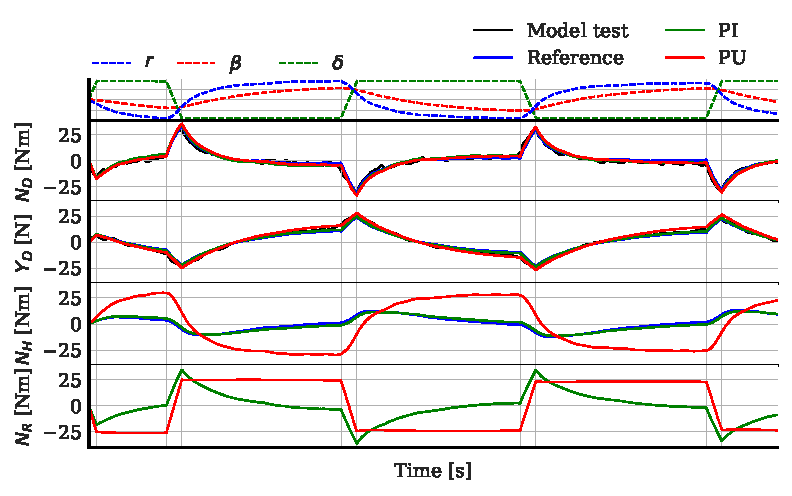
\includegraphics{figures/results.ID_zigzag10.pdf}
    \caption{Inverse dynamics estimations of $Y_D$, and $N_D$ during a zigzag10/10 model test compared with model predictions.}
    \label{fig:ID_zigzag10}
\end{figure}
\begin{figure}[h]
    \centering
    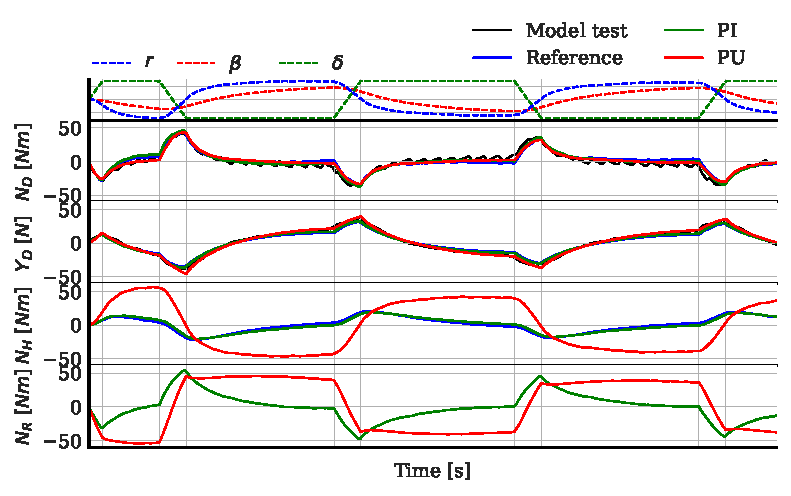
\includegraphics{figures/results.ID_zigzag20.pdf}
    \caption{Inverse dynamics estimations of $Y_D$, and $N_D$ during a zigzag20/20 model test compared with model predictions.}
    \label{fig:ID_zigzag20}
\end{figure}
\FloatBarrier
The hull force model can be closer examined by decomposing the individual parameter contributions. \autoref{fig:ID_regression_N_decomposition} shows the parameter decomposition for the two models together with the reference model. The graphs show the joined contributions for parameters related to drift, and yaw rate. It seems that PI model and the reference model have very similar parameter decompositions.
The parameter decomposition of the PU model is completely different, where almost the entire contribution to the hull yawing moment $N_H$ can be denoted to the yaw rate parameters; The sway force due to drift is also very large.  
\begin{figure}[h]
    \begin{center}
        \includesvg{figures/results.hull_force_decomposition_zigzag20.svg}
        \caption{Decomposition of hull forces and moments during a zigzag20/20 test for parameters related to drift, yaw rate the prediction models.}
        \label{fig:ID_regression_N_decomposition}
    \end{center}
\end{figure}
Possible implications of this physically incorrect decomposition is further investigated in the next section.
\FloatBarrier
%
\subsection{Predictions of an idealized wind state}
\label{sec:idealized_wind_state}
Predictions have been conducted for an idealized wind state, in order to assess the generalization of the  identified models. The idealized wind state is a very simplified hydrodynamic condition where the models have a drift angle, but no yaw rate, or rudder angle; This is meant to represent a state where the ship is experiencing a static drift angle for a long time -- induced by a side wind force.
The prediction results for the idealized wind condition are shown in \autoref{fig:result_wind_state}. The sway force $Y_D$ of the Physics informed model is very similar to the Reference model; For the Abkowitz model the sway force seems to be too large. The yawing moment $N_D$ is under predicted by both models, but the difference is much larger for the Abkowitz model. 
This is because most of the yawing moment is denoted to the yaw rate coefficients (as previously stated in \autoref{sec:result_MDL}) -- which are not activated in the wind state. 
The Physics informed model seems to have a split between the yaw rate and drift angle dependent coefficients that is much more similar to the more physically correct Reference model.
\label{sec:wind_state}
\begin{figure}[h!]
    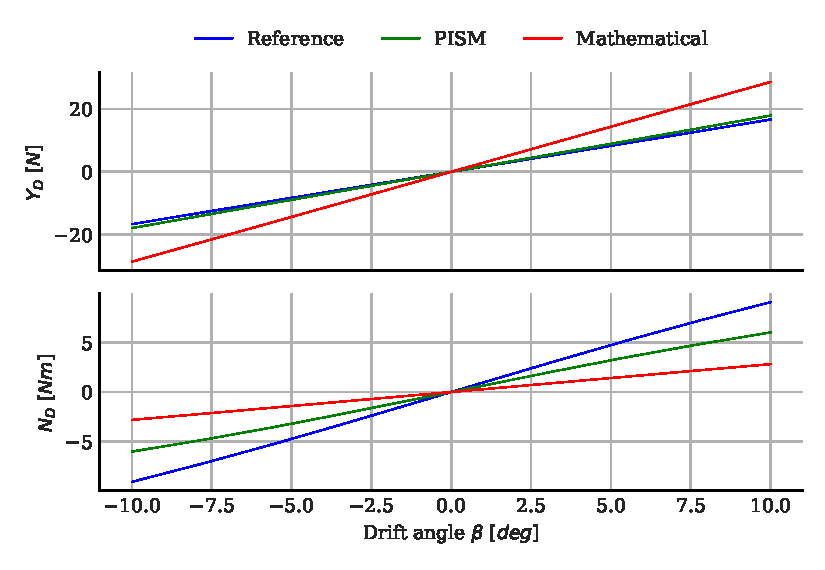
\includegraphics[width=\columnwidth]{figures/result_wind_state.forces.pdf}
    \caption{Total sway force and yawing moment from the models at various drift angles.}
    \label{fig:result_wind_state}
\end{figure}
\FloatBarrier
%
%\section{Discussion}
%\label{sec:discussion}


%
\section{Conclusions}
\label{sec:conclusions}
\begin{itemize}
    \item It was not possible to identify an Abkowitz model that makes sense from a physical point of view based on inverse dynamics forces from the standard manoeuvres used in this paper. This was revealed when the regressed model was compared with the CFD based VCT regression model.
    \item The yawing moment $N_D$ from the Abkowitz model was completely wrong in an idealized wind state.
    \item A pure mathematical model which has been identified on calm water standard manoeuvres can therefore be expected to have a poor generalization into a wind condition.   
    \item The introduction of a semi-empirical rudder model guided the identification toward a more physically correct model, which produced forces that were closer to the VCT reference model. The Physics informed model should therefore have a better generalization into a wind condition.
\end{itemize}
\FloatBarrier

%% The Appendices part is started with the command \appendix;
%% appendix sections are then done as normal sections
\appendix
\section{Hull model}
\label{sec:hull}
The hull forces are expressed with the following general polynomials, which are here expressed in prime system units (see \autoref{sec:prime_system}). The parameters that are omitted in this paper are also indicated. 
\begin{equation}
    \label{eq:X_H}
    {X_H'} = {X_{0}'} + {X_{rr}'} {r'}^{2} + {X_{u}'} {u'} + {X_{vr}'} {r'} {v'} + {X_{vv}'} {v'}^{2}
\end{equation}
%
\begin{equation}
    \label{eq:Y_H}
    {Y_H'} = {Y_{0}'} + {Y_{r}'} {r'} + {Y_{v}'} {v'} + {\cancel{Y_{rrr}}'} {r'}^{3} + {\cancel{Y_{vrr}}'} {r'}^{2} {v'} + {\cancel{Y_{vvr}}'} {r'} {v'}^{2} + {\cancel{Y_{vvv}}'} {v'}^{3}
\end{equation}
%
\begin{equation}
    \label{eq:N_H}
    {N_H'} = {N_{0}'} + {N_{r}'} {r'} + {N_{v}'} {v'} + {\cancel{N_{rrr}}'} {r'}^{3} + {\cancel{N_{vrr}}'} {r'}^{2} {v'} + {\cancel{N_{vvr}}'} {r'} {v'}^{2} + {\cancel{N_{vvv}}'} {v'}^{3}
\end{equation}
%
\section{Rudder models}
\label{sec:rudder_models}
\subsection{Mathematical rudder model}
\label{sec:mathematical_rudder_model}
The mathematical rudder model is expressed as a truncated third order Taylor expansion, similar to \citet{abkowitz_ship_1964}, as seen in \autoref{eq:X_R_math} to \autoref{eq:N_R_math}.
\begin{equation}
    \label{eq:X_R_math}
    {X_R'} = {X_{deltadelta}'} {delta'}^{2}
\end{equation}
%
\begin{equation}
    \label{eq:Y_R_math}
    {Y_R'} = {Y_{deltadeltadelta}'} {delta'}^{3} + {Y_{delta}'} {delta'} + {Y_{rdeltadelta}'} {delta'}^{2} {r'} + {Y_{rrdelta}'} {delta'} {r'}^{2} + {Y_{vdeltadelta}'} {delta'}^{2} {v'} + {Y_{vrdelta}'} {delta'} {r'} {v'} + {Y_{vvdelta}'} {delta'} {v'}^{2}
\end{equation}
%
\begin{equation}
    \label{eq:N_R_math}
    {N_R'} = {N_{deltadeltadelta}'} {delta'}^{3} + {N_{delta}'} {delta'} + {N_{rdeltadelta}'} {delta'}^{2} {r'} + {N_{rrdelta}'} {delta'} {r'}^{2} + {N_{vdeltadelta}'} {delta'}^{2} {v'} + {N_{vrdelta}'} {delta'} {r'} {v'} + {N_{vvdelta}'} {delta'} {v'}^{2}
\end{equation}
\subsection{Semi-empirical rudder model}
\label{sec:semi-empirical_rudder_model}
%\subsubsection{$C_L$}
%\label{sec:CL}
%For a none stalling rudder, the lift coefficient $C_L$ is calculated with \autoref{eq:C_L_semiempirical},
\begin{equation}
    \label{eq:C_L_semiempirical}
    C_{L} = \lambda_{gap} \left(\alpha_} dC_{L dalpha} + \frac{C_{DC} \alpha_} \left|{\alpha_}}\right|}{AR_{e}}\right)
\end{equation}
%
\begin{equation}
    \label{eq:alpha_semiempirical}
    \alpha_{} = \\delta + \gamma_{0 } + \gamma_{}
\end{equation}
The lift slope of the rudder $\frac{\partial C_L}{\partial \alpha}$ is calculated with \autoref{eq:dC_L_dalpha_semiempirical}; 
The effective aspect ratio $AR_e$ accounts for the mirror image effect when the rudder is flush with the hull, where the effective aspect ratio is typically assumed to be twice the geometric aspect ratio $AR_g$ (\autoref{eq:AR_e_semiempirical}) \citep{hughes_tempest_2011}.
The WPCC rudder is however not flush to the hull, so that a gap is created between the rudder and rudder horn for larger rudder angles. This gap reduces the pressure difference between the high and low pressure sides of the rudder in the upper part of the rudder. \citet{matusiak_dynamics_2021} proposes that the gap effect can be modelled as a reduced aspect ratio.
\begin{equation}
    \label{eq:lambda_gap_semiempirical}
    C_{gap} = \begin{cases} 1 & \text{for}\: \delta_{lim} > \left|{\delta}\right| \\s \left(- \delta_{lim} + \left|{\delta}\right|\right)^{2} + 1 & \text{otherwise} \end{cases}
\end{equation}
%

$a_0$ is the section lift curve slope (\autoref{eq:a_0_semiempirical}) and $\Omega$ is the sweep angle of the quarter chord line \citep{lewis_principles_1989}.
\begin{equation}
    \label{eq:dC_L_dalpha_semiempirical}
    dC_{L dalpha} = \frac{AR_{e} a_{0}}{\sqrt{\frac{AR_{e}^{2}}{\cos^{4}{\left(\Omega \right)}} + 4} \cos{\left(\Omega \right)} + 1.8}
\end{equation}
%
\begin{equation}
    \label{eq:AR_e_semiempirical}
    AR_{e} = 2 AR_{g}
\end{equation}
%
\begin{equation}
    \label{eq:AR_g_semiempirical}
    AR_{g} = \frac{b_{R}^{2}}{A_{R}}
\end{equation}
%
\begin{equation}
    \label{eq:a_0_semiempirical}
    a_{0 } = 1.8 \pi
\end{equation}
There is also a small nonlinear part to $C_L$ called $C_{DC}$ which is calculated for a rudder with squared tip using \autoref{eq:C_D_crossflow_semiempirical} where the taper ratio $\lambda$ is defined as the ratio between the chords at the tip and the root of the rudder (\autoref{eq:lambda__semiempirical}) \citep{hughes_tempest_2011}. 
\begin{equation}
    \label{eq:C_D_crossflow_semiempirical}
    C_{DC} = 1.6 \lambda^{} + 0.1
\end{equation}
%
\begin{equation}
    \label{eq:lambda__semiempirical}
    \lambda} = \frac{c_{t}}{c_{r}}
\end{equation}
\subsubsection{$C_D$}
\label{sec:CD}
The drag coefficients for covered $C_{DC}$ and uncovered $C_{DU}$ are calculated with the similar equations: \autoref{eq:C_D_C_semiempirical}, and \autoref{eq:C_D_U_semiempirical}; where $C_{D0C}$ (\autoref{eq:C_D0_C_semiempirical}) and $C_{D0U}$ (\autoref{eq:C_D0_U_semiempirical}) are the drag at zero rudder angle  and $e_0 = 0.9$ is the Oswald efficiency factor. 
\begin{equation}
    \label{eq:C_D_C_semiempirical}
    C_{D C} = C_{D0 C} + \frac{C_{D tune} C_{L}^{2}}{\pi AR_{e} e_{0}}
\end{equation}
%
\begin{equation}
    \label{eq:C_D_U_semiempirical}
    C_{D U } = C_{D0 U } + \frac{C_{D tune} C_{L }^{2}}{\pi AR_{e } e_{0}}
\end{equation}
%
\begin{equation}
    \label{eq:C_D0_C_semiempirical}
    C_{D0 C} = 2.5 C_{D0 tune} C_{F C}
\end{equation}
%
\begin{equation}
    \label{eq:C_D0_U_semiempirical}
    C_{D0 U} = 2.5 C_{D0 tune} C_{F U}
\end{equation}
$C_{D0C}$ and $C_{D0U}$ will be different due to different Reynolds number $Re$ as seen in \autoref{eq:C_F_C_semiempirical} to \autoref{eq:Re_F_U_semiempirical}.
\begin{equation}
    \label{eq:C_F_C_semiempirical}
    C_{F C} = \frac{0.075 \log{\left(10 \right)}^{2}}{\log{\left(Re_{F C} - 2 \right)}^{2}}
\end{equation}
%
\begin{equation}
    \label{eq:C_F_U_semiempirical}
    C_{F U } = \frac{0.075 \log{\left(10 \right)}^{2}}{\log{\left(Re_{F U } - 2 \right)}^{2}}
\end{equation}
%
\begin{equation}
    \label{eq:Re_F_C_semiempirical}
    Re_{F C} = \frac{V_{R C} c_}}{\nu}
\end{equation}
%
\begin{equation}
    \label{eq:Re_F_U_semiempirical}
    Re_{F U} = \frac{V_{R U} c_}}{\nu}
\end{equation}
\subsubsection{Velocity in the propeller slip stream}
\label{sec:velocity_in_the_propeller_slip_stream}
According to momentum theory, the mean axial flow velocity far downstream of the propeller $V_{\infty}$ is given by \autoref{eq:V_infty_semiempirical} \citep{brix_manoeuvring_1993}, in which the thrust coefficient $C_{Th}$ is calculated with \autoref{eq:C_Th_semiempirical}, where $r_0$ is the propeller radius and the apparent velocity $V_A$ is given by \autoref{eq:V_A_semiempirical}.
\begin{equation}
    \label{eq:V_infty_semiempirical}
    V_{\infty } = V_{A } \sqrt{C_{Th } + 1}
\end{equation}
%
\begin{equation}
    \label{eq:C_Th_semiempirical}
    C_{Th } = \frac{2 T_{}}{\pi V_{A }^{2} r_{0}^{2} \rho}
\end{equation}
%
\begin{equation}
    \label{eq:V_A_semiempirical}
    V_{A} = u \left(1 - w_{f}\right)
\end{equation}

The radius of the propeller slipstream far behind the propeller is given by \autoref{eq:r_infty_semiempirical}.
\begin{equation}
    \label{eq:r_infty_semiempirical}
    r_{\infty } = r_{0} \sqrt{\frac{V_{A }}{2 V_{\infty }} + \frac{1}{2}}
\end{equation}
The velocity and the radius of the propeller slipstream at the position of the rudder can be calculated with \autoref{eq:V_x_C_semiempirical} and \autoref{eq:r_p_semiempirical}, respectively, where $x$ is the distance between the propeller and the rudder.
\begin{equation}
    \label{eq:V_x_C_semiempirical}
    V_{x C } = \frac{V_{\infty } r_{\infty }^{2}}{r_{x }^{2}}
\end{equation}
%
\begin{equation}
    \label{eq:r_p_semiempirical}
    r_{x } = \frac{r_{0} \left(\frac{r_{\infty } \left(\frac{x}{r_{0}}\right)^{1.5}}{r_{0}} + \frac{0.14 r_{\infty }^{3}}{r_{0}^{3}}\right)}{\left(\frac{x}{r_{0}}\right)^{1.5} + \frac{0.14 r_{\infty }^{3}}{r_{0}^{3}}}
\end{equation}
Turbulent mixing of the slipstream and the surrounding flow will increase the radius $r_x$ by $r_\Delta$(\autoref{eq:r_Delta_semiempirical}) so that a corrected axial velocity $V_{xcorr}$ can be calculated according to \autoref{eq:V_x_corr_semiempirical}.
\begin{equation}
    \label{eq:r_Delta_semiempirical}
    r_{\Delta } = \frac{0.15 x \left(- V_{A } + V_{x C }\right)}{V_{A } + V_{x C }}
\end{equation}
%
\begin{equation}
    \label{eq:V_x_corr_semiempirical}
    V_{x corr } = V_{A } + \frac{r_{x }^{2} \left(- V_{A } + V_{x C }\right)}{\left(r_{\Delta } + r_{x }\right)^{2}}
\end{equation}
For a twin screw ship a small contribution from the yaw rate is also added to the velocity as seen in \autoref{eq:V_R_x_C_semiempirical}.
\begin{equation}
    \label{eq:V_R_x_C_semiempirical}
    V_{R x C} = V_{x corr} - r y_{R}
\end{equation}
The velocity for the covered part of the rudder is obtained by \autoref{eq:V_R_C_semiempirical}.
\begin{equation}
    \label{eq:V_R_C_semiempirical}
    V_{R C} = \sqrt{V_{R x C}^{2} + V_{R y}^{2}}
\end{equation}
In addition, $V_{xcorr}$ is used to calculate the lift diminished factor $\lambda_R$ together with the expressions in  \autoref{eq:lambda_R_semiempirical}--\autoref{eq:c_semiempirical}.
\begin{equation}
    \label{eq:lambda_R_semiempirical}
    \lambda_{R } = \left(\frac{V_{A }}{V_{x corr }}\right)^{f_{}}
\end{equation}
%
\begin{equation}
    \label{eq:f_semiempirical}
    f_} = \frac{512}{\left(2 + \frac{d_}}{c_}}\right)^{8}}
\end{equation}
%
\begin{equation}
    \label{eq:d_semiempirical}
    d_{} = \frac{\sqrt{\pi} \left(r_{\Delta } + r_{p }\right)}{2}
\end{equation}
\begin{equation}
    \label{eq:c_semiempirical}
    c_} = \frac{c_{r}}{2} + \frac{c_{t}}{2}
\end{equation}
\subsubsection{Velocity outside the propeller slip stream}
\label{sec:velocity_outside_the_propeller_slip_stream}
The axial velocity outside the propeller slip stream $V_{xU}$ equals the apparent velocity (\autoref{eq:V_x_U_semiempirical}). A small contribution from the yaw rate is also added for twin screw ships (\autoref{eq:V_R_x_U_semiempirical}) so that the velocity outside the slip stream can be calculated with \autoref{eq:V_R_U_semiempirical}.
\begin{equation}
    \label{eq:V_x_U_semiempirical}
    V_{x U } = V_{A }
\end{equation}
%
\begin{equation}
    \label{eq:V_R_x_U_semiempirical}
    V_{R x U } = V_{x U } - r y_{R}
\end{equation}
%
\begin{equation}
    \label{eq:V_R_U_semiempirical}
    V_{R U } = \sqrt{V_{R x U }^{2} + V_{R y }^{2}}
\end{equation}

\FloatBarrier
%% If you have bibdatabase file and want bibtex to generate the
%% bibitems, please use
%%
\pagebreak
\bibliographystyle{elsarticle-harv}
\bibliography{Paper_3_semiempirical_rudder.bib}

\end{document}

\endinput
%%
%% End of file `elsarticle-template-harv.tex'.
